\documentclass[12pt]{article}
\usepackage[utf8]{inputenc}
\usepackage{geometry}
\geometry{letterpaper, margin=0.25in}
\usepackage{graphicx} 
\usepackage{parskip}
\usepackage{booktabs}
\usepackage{array} 
\usepackage{paralist} 
\usepackage{verbatim}
\usepackage{subfig}
\usepackage{fancyhdr}
\usepackage{sectsty}
\usepackage[shortlabels]{enumitem}

\pagestyle{fancy}
\renewcommand{\headrulewidth}{0pt} 
\lhead{}\chead{}\rhead{}
\lfoot{}\cfoot{\thepage}\rfoot{}

%%% ToC (table of contents) APPEARANCE
\usepackage[nottoc,notlof,notlot]{tocbibind} 
\usepackage[titles,subfigure]{tocloft}
\renewcommand{\cftsecfont}{\rmfamily\mdseries\upshape}
\renewcommand{\cftsecpagefont}{\rmfamily\mdseries\upshape} %

\usepackage{amsmath}
\usepackage{amssymb}
\usepackage{mathtools}
\usepackage{empheq}
\usepackage{xcolor}
\usepackage{bbm}
\usepackage{tikz}
\usepackage{pgfplots}
\usepackage{tikz-cd}
\pgfplotsset{compat=1.18}
\usetikzlibrary{intersections, decorations.markings}
\tikzset{
    marking along/.style n args={2}{
        decoration={
                markings, 
                mark=at position #1 with {\arrow{#2}}
        },
        postaction={decorate}
        },
    marking along/.default={0.5}{>}
    wavy/.style={
        decorate,decoration={coil,aspect=0}
     },
    two marks/.style n args={1}{
        decoration={
            markings,
            mark=at position 0.25 with {\arrow{#1}},
            mark=at position 0.75 with {\arrow{#1}}
         },
         postaction={decorate}
    }
}

\colorlet{mygreen}{green!50!teal}

\newcommand{\ans}[1]{\boxed{\text{#1}}}
\newcommand{\vecs}[1]{\langle #1\rangle}
\renewcommand{\hat}[1]{\widehat{#1}}

\renewcommand{\P}{\mathbb{P}}
\newcommand{\R}{\mathbb{R}}
\newcommand{\E}{\mathbb{E}}
\newcommand{\Z}{\mathbb{Z}}
\newcommand{\N}{\mathbb{N}}
\newcommand{\Q}{\mathbb{Q}}
\newcommand{\C}{\mathbb{C}}

\newcommand{\ind}{\mathbbm{1}}
\newcommand{\qed}{\quad \blacksquare}

\newcommand{\brak}[1]{\left\langle #1 \right\rangle}
\newcommand{\bra}[1]{\left\langle #1 \right\vert}
\newcommand{\ket}[1]{\left\vert #1 \right\rangle}

\newcommand{\abs}[1]{\left\vert #1 \right\vert}
\newcommand{\mfX}{\mathfrak{X}}
\newcommand{\ep}{\varepsilon}

\newcommand{\Ec}{\mathcal{E}}
\newcommand{\Nc}{\mathcal{N}}
\newcommand{\A}{\mathcal{A}}
\newcommand{\F}{\mathcal{F}}
\newcommand{\Cc}{\mathcal{C}}
\newcommand{\B}{\mathcal{B}}
\newcommand{\M}{\mathcal{M}}
\newcommand{\X}{\chi}
\renewcommand{\L}{\mathcal{L}}

\newcommand{\sub}{\subseteq}
\newcommand{\st}{\text{ s.t. }}
\newcommand{\card}{\text{card }}
\renewcommand{\div}{\vspace*{10pt}\hrule\vspace*{10pt}}
\newcommand{\surj}{\twoheadrightarrow}
\newcommand{\inj}{\hookrightarrow}
\newcommand{\biject}{\hookrightarrow \hspace{-8pt} \rightarrow}
\renewcommand{\bar}[1]{\overline{#1}}
\newcommand{\overcirc}[1]{\overset{\circ}{#1}}
\newcommand{\diam}{\text{diam }}
\newcommand{\iid}{\overset{	ext{iid}}{\sim}}

\renewcommand{\Re}{\text{Re}\,}
\renewcommand{\Im}{\text{Im}\,}
\newcommand{\Var}{\text{Var}\,}
\newcommand{\Cov}{\text{Cov}\,}

\DeclareMathOperator*{\argmax}{\arg\max}
\DeclareMathOperator*{\argmin}{\arg\min}

\newcommand{\sign}{\text{sign}\,}

\newcommand*{\tbf}[1]{\ifmmode\mathbf{#1}\else\textbf{#1}\fi}

\usepackage{tcolorbox}
\tcbuselibrary{breakable, skins}
\tcbset{enhanced}
\newenvironment*{tbox}[2][gray]{
    \begin{tcolorbox}[
        parbox=false,
        colback=#1!5!white,
        colframe=#1!75!black,
        breakable,
        title={#2}
    ]}
    {\end{tcolorbox}}

\newenvironment*{exercise}[1][red]{
    \begin{tcolorbox}[
        parbox=false,
        colback=#1!5!white,
        colframe=#1!75!black,
        breakable
    ]}
    {\end{tcolorbox}}

\newenvironment*{proof}[1][blue]{
\begin{tcolorbox}[
    parbox=false,
    colback=#1!5!white,
    colframe=#1!75!black,
    breakable
]}
{\end{tcolorbox}}
\newenvironment*{proposition}[1][gray]{
    \begin{tcolorbox}[
        parbox=false,
        colback=#1!5!white,
        colframe=#1!75!black,
        breakable
    ]}
    {\end{tcolorbox}}

\title{APMA 1360: Homework 10}
\author{}
\date{}
\begin{document}
\maketitle

\vspace{-1in}
\section{The tent map is chaotic}

Define the tent map via

\centerline{%
    \raisebox{1,2cm}{$T(x) := \left\{\begin{array}{lcl}
                2x   & \mbox{for} & 0\leq x\leq\frac12  \\
                2-2x & \mbox{for} & \frac12\leq x\leq1.
            \end{array}\right.$} \qquad
    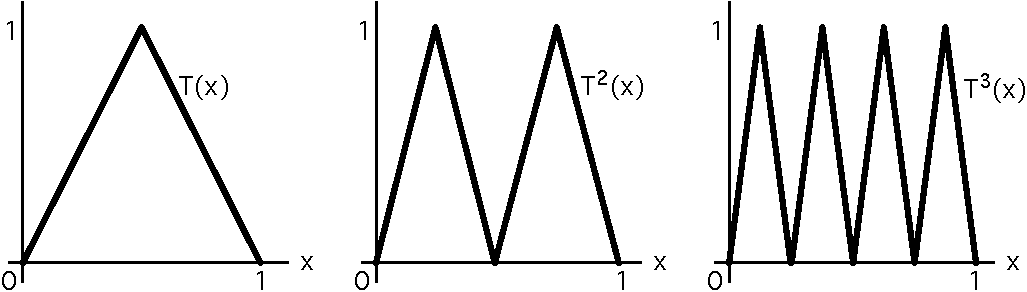
\includegraphics[scale=0.6]{Assignment_Figure_8}}
\begin{enumerate}[(i)]
    \item Compute the Lyapunov exponent $\ell(x_0)$ of the tent map for each $x_0\in[0,1]$.

          \color{blue}
          We define
          \[ \ell(x_0) = \lim_{n \to \infty} \frac{1}{n} \sum_{j=0}^{n-1} \log \abs{T'(x_j)} \]


          Since
          \[T'(x) = \begin{cases}
                  2  & \text{if } 0\leq x\leq \frac{1}{2} \\
                  -2 & \text{if } \frac{1}{2} < x\leq 1
              \end{cases}\]
          we have
          \[\ell(x_0) = \lim_{n \to \infty} \frac{1}{n} \sum_{j=0}^{n-1} \log 2 = \boxed{\log 2}\]

          \color{black}

    \item Argue that the graph of $T^n$ consists of $2^{n-1}$ tents as indicated in the figure for $n=2,3$. Hint: Show this first for $T^2$; then, assuming that you know that $T^n$ consists of $2^{n-1}$ tents, show that $T^{n+1}$ has $2^n$ tents: each line segment of $T^n$ becomes another tent, since the image of the line segment is the entire interval $[0,1]$ on which $T$ looks like a tent.

          \color{blue}
          First consider $T^2$. Since $T$ is a piecewise double cover of $[0, 1]$, we can write
          \[T([0, 1]) = I^+ \cup I^- \cong [0,1]^2\]
          where $I^+$ is the component of the image of $T$ with positive slope and $I^-$ is the component with negative slope.

          Then, $T^2([0, 1]) = T(I^+) \cup T(I^i)$. Each $T$ maps the interval $[0, 1] \cong I^+ \cong I^-$ into a tent, so $T^2$ maps the interval into two tents.

          In fact, we could see this directly:
          \[T^2(x) = \begin{cases}
                  4x     & 0 \leq x \leq 1/4 \\
                  2 - 4x & 1/4 < x \leq 1/2  \\
                  4x - 2 & 1/2 < x \leq 3/4  \\
                  4 - 4x & 3/4 < x \leq 1    \\
              \end{cases}\]
          which corresponds to four line segments, two with positive slope and two with negative slope.

          Suppose now that $T^n$ consists of $2^{n-1}$ tents. Let $I_j = I_j^+ \cup I_j^-$ be the $j$-th tent and $I_j^+$ and $I_j^-$ be its positive and negative slope components, each of which is isomorphic to $[0, 1]$.

          Therefore, we can write
          \[T^n([0, 1]) = \bigcup_{j=1}^{2^{n-1}} I_j^+ \cup I_j^-\]
          hence
          \[T^{n+1}([0, 1]) = T\left(\bigcup_{j=1}^{2^{n-1}} I_j^+ \cup I_j^-\right) = \bigcup_{j=1}^{2^{n-1}} T(I_j^+) \cup T(I_j^-)\]
          but each $T(I_j)^+$ and $T(I_j)^-$ is a tent, so we could reindex by
          \[T^{n+1}([0, 1]) = \bigcup_{k=1}^{2^{n}} I_k\]
          where $I_k$ is the $k$-th tent.
          \color{black}

    \item Use this characterization of $T^n$ to show that there are $2^n$ points in the interval for which $T^n(x)=x$. Show also that the set of periodic orbits of the tent map is dense in the interval $[0,1]$.

          \color{blue}
          From the previous part, we know that $T^n$ consists of $2^{n-1}$ tents. Each tent is composed of two line segments, yielding $2^n$ total line segments $I_j$. Notice that $T^n: I_j \to [0, 1]$ is a surjection. Since $I_j \sub [0, 1]$, we can find at least one point $x_j \in I_j$ such that $T^n (x_j) = x_j$ for each $j=1: 2^n$.

          Therefore, it suffices to show that each interval contains exactly one fixed point.

          Suppose on the contrary that $\exists I_j$ such that $T^n(x_1) = x_1$ and $T^n(x_2) = x_2$ for $x_1 \neq x_2$. WLOG let $x_2 > x_1$ and $x_1 + \ep = x_2$.

          Note, though, that $T^n$ is continuous and strictly monotonic on each $I_j$. If $\frac{d}{dx}\big\vert_{x_1} T^n < 0$, then $x_1 = T^n(x_1) > T^n(x_2) = x_2$, which is a contradiction.

          Hence, we could only have two fixed points for $I_j$ where $\frac{d}{dx}T^n > 0$. In this case, since $T^n \big\vert_{I_j}$ is linear,
          \begin{align*}
              T^n(x_2)  & = T^n(x_1) + \frac{d}{dx}T^n(x_1)(x_2 - x_1)   \\
              x_2       & = x_1 + \frac{d}{dx}T^n(x_1)(x_2 - x_1)        \\
              x_1 + \ep & = x_1 + \frac{d}{dx}T^n(x_1) (x_1 + \ep - x_1) \\
              \ep       & = \ep \frac{d}{dx}T^n(x_1)                     \\
              1         & = \frac{d}{dx}T^n(x_1)                         \\
          \end{align*}
          for all $n$ and all $x_1 \in I_j$.

          Trivially, however, this fails already on $n=1$ since, on its positive component, $\frac{d}{dx} T^1(x) = 2 \neq 1$.

          Hence, we conclude that $T^n$ has exactly one fixed point in each of the $2^n$ intervals $I_j$, yielding $2^n$ fixed points on $[0, 1]$.

          \div

          Let $P_k = \{x \in [0, 1]: T^k(x) = x\}$ be the set of points (with not necessarily smallest) period $k$ and $P = \bigcup_{k=1}^{\infty} P_k$ be the set of all periodic points.

          We showed above that $\abs{P_k} = 2^k$ for all $k \geq 1$. Further, by construction,
          \[\exists p_j \in P_k: p_j \in I_j = \left[\frac{j}{2^k}, \frac{j+1}{2^k}\right], \quad j=0: 2^k - 1\]

          By density of the rationals, for all $\ep > 0$ and any $x \in [0, 1]$, we can construct a neighborhood $x \in \left[\frac{j}{2^k}, \frac{j+1}{2^k}\right]$ for $k$ sufficiently large such that $\abs{p_j - x} < \ep$ with $p_j \in P_k$.

          Hence, the set of periodic orbits is dense in $[0, 1]$.

          \color{black}

\end{enumerate}
It is also possible to show that the tent map is topologically transitive and has a dense orbit: together with the statements you proved above, this shows that the tent map is chaotic!

\pagebreak

\section{The logistic map is chaotic}

Let $f_1(x)$ and $f_2(x)$ be two maps from the interval $[0,1]$ into itself. We say that $f_1$ and $f_2$ are conjugate if there is a map $h:[0,1]\to[0,1]$ that is continuous, 1-1, and onto so that $f_1\circ h=h\circ f_2$ or $f_1(h(x))=h(f_2(x))$ for all $x\in[0,1]$.
\begin{enumerate}[(i)]
    \item Argue that this implies that $f_1^n(x)=h\circ f_2^n\circ h^{-1}$ or $f_1^n(x)=h(f_2^n(h^{-1}(x)))$ for all $x\in[0,1]$ and all $n\geq1$. In particular, the dynamics of $f_1$ and $f_2$ are the same.

          \color{blue}
          Suppose $f_1(h(x)) = h(f_2(x))$ for all $x\in[0,1]$. Then, since $h^{-1}(x)$ is well-defined for all $x \in [0,1]$,
          \[f_1(h(h^{-1}(x))) = h(f_2(h^{-1}(x))) \implies f_1(x) = h(f_2(h^{-1}(x)))\]

          Now consider $f_1^2(x)$:
          \[f_1(f_1(x)) = h(f_2(h^{-1}(h(f_2(h^{-1}(x)))))) = h(f_2^2(h^{-1}(x)))\]
          as desired.

          Suppose that $f_1^n(x) = h(f_2^n(h^{-1}(x)))$ for all $x\in[0,1]$ and all $n\geq1$. Then,
          \[f_1^{n+1}(x) = f_1(f^n(x)) = h(f_2(h^{-1}(h(f_2^n(h^{-1}(x)))))) = h(f_2^{n+1}(h^{-1}(x)))\]
          \color{black}

    \item Show that the tent map and the logistic map $f(x)=4x(1-x)$ are conjugate on $[0,1]$. More precisely, with $h(x)=\sin^2(\pi x/2)$ (the square of the sine function), show that $f(h(x))=h(T(x))$ for all $x\in[0,1]$. Use \#10.1 to conclude that the logistic map is chaotic.

          \color{blue}
          \begin{align*}
              f(h(x)) & = 4\sin^2(\pi x/2)(1 - \sin^2(\pi x/2))          \\
                      & = 4\sin^2(\pi x/2)\cos^2(\pi x/2)                \\
                      & = \frac{4(1 - \cos (2\pi x))}{8}                 \\
                      & = \frac{1- \cos(2\pi x)}{2}                      \\
                      & = \frac{1 - (1 - 2\sin^2(\pi x))}{2}             \\
                      & = \sin^2(\pi x)                                  \\
                      & = \begin{cases}
                              \sin^2(\pi x)      & 0 \leq x \leq \frac{1}{2} \\
                              \sin^2(\pi(1 - x)) & \frac{1}{2} < x \leq 1
                          \end{cases} \\
                      & = h(T(x))
          \end{align*}

          In \#10.1, we showed that the tent map is chaotic. Since the logistic map is conjugate to the tent map (that is, their dynamics are the same), we conclude that the logistic map is also chaotic.
          \color{black}

\end{enumerate}

\end{document}